\documentclass[10pt,twoside]{article}
%\usepackage[a4paper,top=0.9in, bottom=2.54cm, vscale=1, left=0.75in, right=0.75in]{geometry}
\addtolength{\oddsidemargin}{-.875in}
	\addtolength{\evensidemargin}{-.875in}
	\addtolength{\textwidth}{1.75in}

	\addtolength{\topmargin}{-.875in}
	\addtolength{\textheight}{1.75in}
\usepackage[a4paper,vscale=0.8]{geometry}
\usepackage[british]{babel}
\usepackage[utf8]{inputenc}
\usepackage{amsmath}
\usepackage{graphicx}
\usepackage{parskip}
%\usepackage{natbib}
\usepackage{pgfgantt}
\usepackage{lscape}
\usepackage{tabularx}
\usepackage{pdfpages}
\usepackage{graphicx}
\usepackage{xcolor}
\usepackage[listingsutf8,minted]{tcolorbox}
\usepackage{hyperref}
\usepackage[chapter]{tocbibind}
\usepackage{doc}
\usepackage{minted}
\usepackage{listings}
\usepackage{listingsutf8}
\usepackage[colorinlistoftodos]{todonotes}

\usepackage{enumitem}
\usepackage[style=authoryear-ibid,backend=biber]{biblatex}
\addbibresource{writing.bib}

\title{Using website log files to detect low bandwidth attacks through the application of heuristic analysis. \\
\small Chapter 2 - draft updated \today}

\author{Peter Smith \\
\small Supervisor - Nick Dalton\\
\small 2nd Marker - Neil Eliot
}

\includepdfset{pagecommand={}}
\includepdfset{width=\textwidth}
\begin{document}
\maketitle
%!TeX root=Dissertation.tex

\section*{Introduction}
This chapter will look at the various types of attacks that can occur on websites. Some of these attacks are more serious in nature in comparison to others, a selection of attacks will be looked at and the detection and prevention of these attacks will be analysed; this will feed into the final product, so that the product can display a risk analysis to the users.  The main two attacks looked at will be  low-bandwidth attacks and SQL injection attacks as well as Other common attacks
%!TeX root=Dissertation.tex

\section{Low-bandwidth attacks} \label{attack1}

In order to comprehend the nature of the topic, and the difficulty in detecting Low-bandwidth attacks some other fundamental concepts should be illustrated within the body of this introduction for supplemental understanding of many of the research methods discussed.

A paper written by Adi 2017 uses a SYN flag variable as a benchmark for threat detection; to understand this variable the mechanics of a TCP connection must be described. TCP is a connection-oriented protocol, a connection needs to be established before two devices can communicate. TCP uses a process called three-way handshake to negotiate the sequence and acknowledgment fields and start the session. Two devices would be in communication, the Client and the Server. The Client initiates the connection by sending the TCP SYN (SYNchronize) packet to the destination Server and the Server receives the packet and responds with an acknowledgement. The Client then acknowledges the response of the Server by sending the acknowledgment back, and a connection is formed. 

A low-rate and low bandwidth attack is a different kind of attack in comparison to a normal DoS attack. A DoS attack works on overwhelming the server with requests, therefore it is easier to detect than a low-rate attack, for example, if you receive a large amount of traffic from a single IP; this is more than likely a DoS attack (REF NEEDED). A normal internet request operates based on an HTTP GET request to the web server that allows access to the site, the outcome of a DoS attack is the creation of a disruption between the clients and the web host. High-bandwidth attacks will keep trying to request multiple web pages at the same time to overwhelm the server however, a low-bandwidth attack sends a partial request and then may wait 20-30 seconds for example, it then sends new data, just enough to keep the connection open. One type of a Low-bandwidth attack is a slow loris attack; this is a layer-7 application attack, that only requires a small level of band-width and thus means the attacker can have continual use over their system and carry out normal activity. A web server will have a set number of sockets that it can have open at any one time, for this explanation we will choose to use 10 sockets. The aim of a slow loris is to open all 10 sockets and keep them busy, therefore, no new sockets can be opened and thus, no client interaction will take place. The difficulty with detecting these types of attacks is that the legitimate user may just have a slow internet connection thus, making distinguishing these attacks from slow users difficult. 

\subsection{Attack Detection Techniques}

Work done by Adi and Tripathi shows that even though HHTP/2, defined as RCF 7540, is a more  modern protocol, than that of HTTP/1.1, defined as  RCF 2616. Tripathi suggests that HTTP/2 has more threat vectors (\cite{tripathi2018slow}). Adi also notes that "The HTTP/2-standard states that if the host machine does not monitor resource usage, it exposes itself to a risk of a DoS attack" (\cite{Adi2015}).

The largest amount of research done into Low rate Dos attacks is by Erwin Adi, Zubair Baig, Chiou Peng Lam, and Phillip Hingston their work started in 2015 and have 3 papers on this subject, the last of which was 2018. The majority of their work looked at using resource utilisation in order to detect Low bandwidth attacks. They set numerous tests to analyse the behaviours of victim machines when subject to Low rate Dos Attacks. 

The 2016 study carried out 4 varying investigations to analyse the behaviour of a victim machine when subject to large volume low rate DoS attacks. The researchers used a flood of windows PING and WINDOWS UPDATE frames to Simulate a Low-Rate DoS attack on a server, and demonstrated how legitimate HTTP/2 Flash Crowd could be launched to create a DoS scenario.  The team noted at the time of their 2016 investigation there was no reported study to ascertain whether or not attack traffic could be concealed in a stealthy manor to appear as legitimate Flashcrowd traffic. The research concluded that the HTTP/2 protocol itself does not restrict the intensity of traffic generated, and that auxiliary mechanisms should be implemented for identifying volumes and patterns of network traffic. (\cite{Adi2016}) Trapathi stated as criticism in his 2018 study that both the 2015 and 2016 study completed by Adi's team that neither experiment managed to achieve a completed exhaustion of computational resource (\cite{tripathi2018slow}) Therefore it could be argued that Adi's research did not represent the full effect of a DoS attack. When looking into detail of the results from Adi's research, the figures quoted in Table 1 in the paper by Adi, the figures show depletion rates of between 88.39\% to 98.56\% (\cite{Adi2016}). Due to the ineffective depletion of the CPU the majority of his detection methods should be questioned as Trapathi points out....Even Erwin Adi himself points out that his methodology could potentially be flawed.....(5.2) Therefor Adi's proposed method for monitoring CPU depletion as a way to detect low rate bandwidth attacks could be fundamentally flawed. Adi's study was done on a server with one single website and did not run any other background services for example, email, which would in theory add unpredictable CPU loads and make his detection method difficult to implement.

\begin{wrapfigure}{R}{}
\label{addie table}
    \centering
    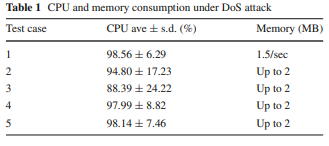
\includegraphics{Apdenix/adiTable.PNG}
    \caption{Table 1 from \cite{adi2017stealthy}}
    \label{fig:my_label}
\end{wrapfigure}
Although Adi's 2016 work looked at HTTP/2 it was noted in their later 2017 paper that 90\% of contemporary web servers as to the date of that study had not yet migrated to HTTP/2 from HTTP/1.x (\cite{adi2017stealthy}) At the time of this paper November 2019, HTTP/2 was used by 41.7\% of the top 10 million websites (\cite{w3techs}), as seen in figure 2 below. This illuminates the pressing need for research into the assailability of the HTTP/2 protocol and consequent detection methods and fixes. 

\begin{wrapfigure}{L}{}
\label{web using h2}
    \centering
    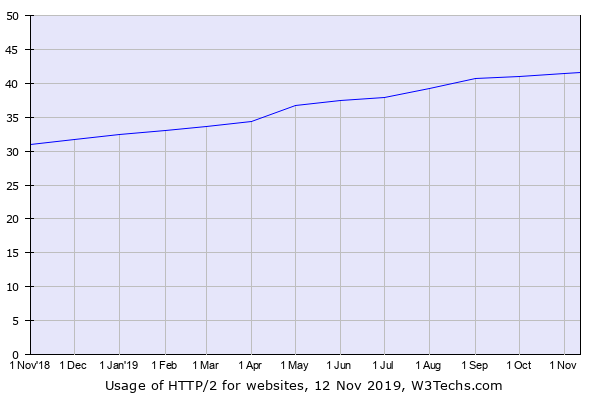
\includegraphics[width=88mm,scale=0.8]{Apdenix/HTTP2SITESgraph.png}
    \caption{Usage of HTTP/2 for Websites, 12 Nov 2019, W3Techs.com}
    \label{web http2}
\end{wrapfigure}
Adi's 2017 work looked at some of the stealthier approaches that cyber attacks were using in order to bypass current detection methods. Adi and his team set up two models intended to simulate stealthy Low rate DoS attacks which they called 'bots'. The investigation aimed to model attacks whose traffic continually consumed the victims computing resource, while still being stealthy enough to yield some false alarms via the target servers' 'learning' mechanisms. Adi constructed the attack 'bots' with four core factors for experimentation, these were number of threads, number of window\_update, stealthy factor and delay between successive TCP connections. These two sets of Stealth models were tested against regular flash crowd traffic in an effort to differentiate the pattern. The experiment and subsequent analysis was successful in distinguishing a notable difference in the patterns of the number of packets carrying SYN flags per 1-second traffic instance between regular flashcrowd traffic and the simulated stealthy attacks. (\cite{adi2017stealthy}) Since Adi's work there appears to be an implementation of the methodology proposed in their paper. Cloudflare have been able to implement a defence mechanism against a SYN flood attack. The have created a program called 'gatebot' which monitors SYN packet packet requests and attempts to drop malicious SYN packets on the firewall layer. (\cite{CFSYN})

Tripathi's 2018 study, however, took a sample of websites and attempted to detect Low rate attacks by monitoring benchmarking by measuring the Chi squared (X\textsuperscript{\small2}) differential value between the expected and observed traffic pattern. Tripathi suggests this approach could detect attacks with high accuracy and may lead to further research to assess further HTTP/2 vulnerabilities and potentially mitigating these threat vectors with fixes. Trapathi indicated that although his detection method for attack traffic was successful; if HTTP/2 traffic data is encrypted it must then be decrypted before submitting traces to the detector. He suggested that this could be easily achieved with the aid of an intercepting proxy before forwarding to the target website responsible for handling HTTP/2 requests. It must be noted that most large companies are utilising this strategy to intercept traffic coming into their local network. (\cite{tripathi2018slow}). 
\section{port scanning}

A port scanner attack is a attack whereby an attacker will send packages of information to different ports on a server to see which ports can be accessed; this may lead them to be able to log into different parts of the server using a brute force approach. Some of the standard ports that are use d in a web server are WWW 80, ftp 21 and nameserver 53 (REF NEEDED). SSH 22. A lot of web hosts and sever owners change the ports for SSH and the ftp however, they may inevertinbly (how spell) leave ports open that are not secure. 
READ https://ieeexplore.ieee.org/stamp/stamp.jsp?tp=&arnumber=6122824
\printbibliography
\end{document}